\documentclass[cal1spr16Lectures.tex]{subfiles}

\begin{document}

%\section[Week 10]{Week 10: 28 Mar - 1 Apr}

% % % 
\subsubsection{\bf Friday 1 April}
% % %

\begin{frame}[allowframebreaks]{Fri 1 Apr}
\begin{itemize}%\footnotesize
\item Exam 3: next Friday.  Covers \S 3.10-4.6 
\end{itemize}
\end{frame}

% % %
\subsection[4.5 Linear Approximation and Differentials]{\S 4.5 Linear Approximation and Differentials}
% % %

% % %
\begin{frame}{\S 4.5 Linear Approximation and Differentials}
\footnotesize
Suppose $f$ is a function such that $f^{\prime}$ exists at some point $P$.  If you zoom in on the graph, the curve appears more and more like the tangent line to $f$ at $P$.  

\centering{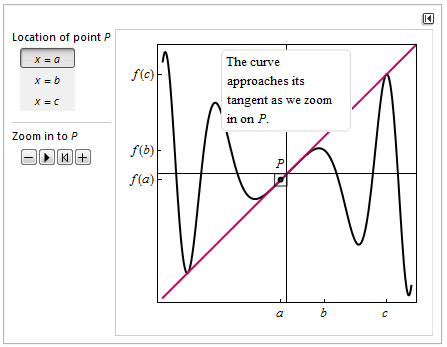
\includegraphics[scale=0.54]{pictures/linApprox}}
\end{frame}

% % %
\subsubsection{Linear Approximation}
% % % 

% % %
\begin{frame}{\small Linear Approximation}
\footnotesize
This idea -- that \alert{smooth} curves (i.e., curves without corners) appear straighter on smaller scales -- is the basis of linear approximations.

\vspace{1pc}
One of the properties of a function that is \alert{differentiable} at a point $P$ is that it is \alert{locally linear} near $P$ (i.e., the curve approaches the tangent line at $P$.)

\vspace{1pc}
Therefore, it makes sense to approximate a function with its tangent line, which matches the value and slope of the function at $P$.  

\vspace{1pc}
This is why you've had to do so many ``find the equation for the tangent line to the given point" problems!
\end{frame}

% % %
\begin{frame}
\frametitle{}
\footnotesize
\begin{dfn} Suppose $f$ is differentiable on an interval $I$ containing the point $a$.  The {\bf linear approximation} to $f$ at $a$ is the linear function
\[L(x)=f(a)+f^{\prime}(a)(x-a)\qquad\text{for $x$ in $I$.}\]
\end{dfn}

\vspace{1pc}
{\bf Remarks:} Compare this definition to the following: At a given point $P=(a,f(a))$, the slope of the line tangent to the curve at $P$ is $f^{\prime}(a)$.  So the equation of the tangent line is
\[y-f(a)=f^{\prime}(a)(x-a).\]

(Yes, it is the same thing!)
\end{frame}

% % %
\begin{frame}
\frametitle{}
\small
\begin{exe} Write the equation of the line that represents the linear approximation to 
\[f(x)=\dfrac{x}{x+1}\qquad\text{ at $a=1$.}\]  
Then {\it use} the linear approximation to estimate $f(1.1)$. \end{exe}

\vspace{1pc}
{\bf Solution:} First compute
\[f^{\prime}(x)=\dfrac{1}{(x+1)^2},\quad f(a)=\dfrac{1}{2},\quad f^{\prime}(a)=\dfrac{1}{4}\]
\[L(x)=\dfrac{1}{2}+\dfrac{1}{4}(x-1)=\dfrac{1}{4}x+\dfrac{1}{4}.\]
\end{frame}

% % %
\begin{frame}
\small
{\bf Solution (continued):}

\bigskip

Because $x=1.1$ is near $a=1$, we can estimate $f(1.1)$ using $L(1.1)$:
$$f(1.1) \approx L(1.1)= 0.525$$

\bigskip

Note that $f(1.1)=0.5238$, so the error in this estimation is
$$\dfrac{0.525-0.5238}{0.5238} \times 100=0.23 \%.$$
\end{frame}

% % %
\begin{frame}
\begin{exe}
\begin{itemize}
\item[(a)] The linear approximatioln to $f(x)=\sqrt{1+x}$ at the point $x=0$ is (choose one):
	\begin{itemize}
	\item[A. ]$L(x)=1$
	\item[B. ]$L(x)=1+\textstyle\frac{x}{2}$
	\item[C. ]$L(x)=x$
	\item[D. ]$L(x)=1-\textstyle\frac{x}{2}$
	\end{itemize}
\item[(b)] What is an approximation for $f(0.1)$?
\end{itemize}
	\end{exe}
\end{frame}

% % %
\subsubsection{Intro to Differentials}
% % %

% % %
\begin{frame}{\small Intro to Differentials}
\small
Our linear approximation $L(x)$ is used to approximate $f(x)$ when $a$ is fixed and $x$ is a nearby point:
\[f(x) \approx f(a)+f^{\prime}(a)(x-a)\]

\vspace{1pc}
When rewritten,
\begin{align*}
f(x)-f(a) & \approx f^{\prime}(a)(x-a) \\[0.5pc]
\implies \Delta y & \approx f^{\prime}(a) \Delta x.
\end{align*}
\end{frame}

% % %
\begin{frame}
\footnotesize
A change in $y$ can be approximated by the corresponding change in $x$, magnified or diminished by a factor of $f^{\prime}(a)$.  

\vspace{1pc}
This is another way to say that $f^{\prime}(a)$ is the rate of change of $y$ with respect to $x$!
\begin{align*}
\Delta y & \approx f^{\prime}(a) \Delta x \\[0.5pc]
\frac{\Delta y}{\Delta x} & \approx f^{\prime}(a)
\end{align*}

\vspace{1pc}
So if $f$ is differentiable on an interval $I$ containing the point $a$, then the change in the value of $f$ (the $\Delta y$), between two points $a$ and $a+\Delta x$ in $I$, is \alert{approximately} $f'(x)\Delta x$. 
\end{frame}

% % %
\begin{frame}
\small
We now have two different, but related quantities:

\begin{itemize}
\item The change in the function $y=f(x)$ as $x$ changes from $a$ to $a+\Delta x$ (which we call $\Delta y$).

\vspace{0.5pc}
\item The change in the linear approximation $y=L(x)$ as $x$ changes from $a$ to $a+\Delta x$ (called the \alert{differential}, $dy$).
\end{itemize}

%\vspace{0.5pc}
\[\Delta y \approx dy\]
\end{frame}

% % %
\begin{frame}
\frametitle{}
\small
When the $x$-coordinate changes from $a$ to $a+\Delta x$:
\begin{itemize}
\item The function change is \underline{{\bf exactly}} $\Delta y=f(a+\Delta x)-f(a)$.
\item The linear approximation change is 
\begin{alignat*}{2}
\Delta L &= L(a+\Delta x)-L(a) \\[0.5pc]
&= \left( f(a)+f^{\prime}(a)(a+\Delta x -a) \right) - \left( f(a)+f^{\prime}(a)(a-a) \right) \\[0.5pc]
&= f^{\prime}(a) \Delta x
\end{alignat*}
and this is $dy$.
\end{itemize}
\end{frame}

% % %
\begin{frame}
\small
We define the differentials $dx$ and $dy$ to distinguish between the \alert{change in the function ($\Delta y$)} and the \alert{change in the linear approximation ($\Delta L$)}: 
\begin{itemize}
\item $dx$ is simply the change in $x$, i.e.\ $\Delta x$.
%\vspace{0.25pc}
\item $dy$ is the change in the linear approximation, which is $\Delta L=f^{\prime}(a) \Delta x$.
\end{itemize}

{\bf SO:}
\begin{align*}
\Delta L &= f^{\prime}(a) \Delta x \\[0.5pc]
dy &= f^{\prime}(a) dx \\[0.5pc]
\dfrac{dy}{dx} &= f^{\prime}(a)\quad \text{ (at $x=a$)}
\end{align*}
\end{frame}

% % %
\begin{frame}
\frametitle{}
\small
\begin{dfn} Let $f$ be differentiable on an interval containing $x$.
\begin{itemize}
\item A small change in $x$ is denoted by the {\bf differential} $dx$.
\item The corresponding change in $y=f(x)$ is \underline{approximated} by the {\bf differential} $dy=f^{\prime}(x)dx$; that is,
\begin{align*}
\Delta y& = f(x+\Delta x)-f(x) \\[0.5pc]
\approx dy &= f^{\prime}(x)dx.
\end{align*}
\end{itemize}
\end{dfn}

\vspace{1pc}
{\bf The use of differentials is critical as we approach integration.}
\end{frame}

% % %
\begin{frame}
\frametitle{}
\small
\begin{ex} Use the notation of differentials $[dy = f^{\prime}(x) dx]$ to approximate the change in $f(x)=x-x^3$ given a small change $dx$. \end{ex}

{\bf Solution:} $f^{\prime}(x)=1-3x^2$, so $dy=(1-3x^2)dx.$

A small change $dx$ in the variable $x$ produces an approximate change of $dy=(1-3x^2)dx$ in $y$.

\vspace{1.5pc}
For example, if $x$ increases from 2 to 2.1, then $dx=0.1$ and 
\[dy=\left(1-3(2)^2 \right)(0.1)=-1.1.\]
This means as $x$ increases by 0.1, $y$ decreases by 1.1.
\end{frame}

% % %
\subsubsection{Book Problems}

% % %
\begin{frame}
\begin{block}{4.5 Book Problems}
13-20, 35-50
\end{block}
\end{frame}

\end{document}